\subsection{Pressurized hollow sphere}
\paragraph{}
The problem is a pressurized hollow sphere subjected to the internal pressure.
The geometry of the problem is described in Fig.\ref{oct_fig:ex_pre-hollow-sphere}. 

\begin{figure}[h!]
  \centering
  \scalebox{1}{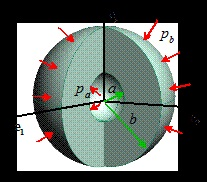
\includegraphics{octree/ex_images/oct_ex_image021.jpg}}
  \caption{Pressurized hollow sphere}
  \label{oct_fig:ex_pre-hollow-sphere}
\end{figure}

\paragraph{}
In the example, the external pressure is set to be zero so that only the internal one is considered.
The geometric properties are: $a=\SI{10}{\meter}$ and $b=\SI{50}{\meter}$.
The boundary condition\hl{s are}: $p_a = \SI{10}{\newton \per \square \meter}$ ,$p_b = 0$ and the rigid body motion is prevented.
The material properties are: $E=\SI{200}{\newton \per \square \meter}$ and $\nu=0.3$.
For simplification, only a quarter of the sphere is analysed as shown in Fig.~\ref{oct_fig:ex_hollow_sphere_mesh_1716}
Analytical surface traction is applied on all of the boundary surfaces.
First order tetrahedral element is adopted to calculated the displacement and \hl{the} stress and they are compared to the exact solution as in Eq.~\ref{oct_eq:ex_hollow_sphere_ana_sol} in spherical coordinate.

\begin{subequations}
\begin{align}
  u & = \frac{1}{2E(b^3-a^3)R^2}\left\{ 2(p_aa^3-p_bb^3)(1-2\nu)R^3+(p_a-p_b)(1+\nu)b^3a^3\right\}\\
  \sigma_{RR} & = \frac{p_aa^3-p_bb^3}{b^3-a^3} - \frac{(p_a-p_b)b^3a^3}{(b^3-a^3)R^3}\\
  \sigma_{\theta\theta} & = \frac{p_aa^3-p_bb^3}{b^3-a^3} + \frac{(p_a-p_b)b^3a^3}{2(b^3-a^3)R^3}\\
  \sigma_{\phi\phi} & = \sigma{\theta\theta}
  \label{oct_eq:ex_hollow_sphere_ana_sol}
\end{align}
\end{subequations}
The tensor transformation from spherical coordinate to cartesian coordinate can be written as Eq.~\ref{eqn:transformation} according to Fig.~\ref{octree_fig:oct_ex_hollow_sphere_tran}.
\begin{subequations}
  \begin{align}
    \begin{bmatrix}
      S_{xx} & S_{xy} & S_{xz} \\
      S_{xy} & S_{yy} & S_{yz} \\
      S_{xz} & S_{yz} & S_{zz} \\
    \end{bmatrix} = T\begin{bmatrix}
      S_{RR} & S_{R\theta} & S_{R\phi} \\
      S_{R\theta} & S_{\theta\theta} & S_{\theta\phi}\\
      S_{R\phi} & S_{\theta\phi} & S_{\phi\phi} \\
    \end{bmatrix} T^T\\
  T = 
\begin{bmatrix}
\sin\theta\cos\phi & \cos\theta\cos\phi & -\sin\phi \\
\sin\theta\sin\phi & \cos\theta\sin\phi & \cos\phi  \\
\cos\theta & -\sin\theta & 0 \\
\end{bmatrix}
\end{align}
\label{eqn:transformation}
\end{subequations}
%
\begin{figure}[h!]
    \centering
    \scalebox{0.5}{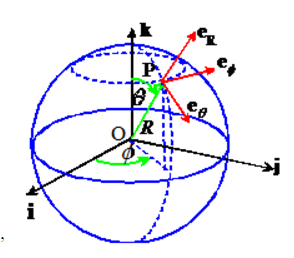
\includegraphics{octree/ex_images/oct_ex_tran.png}}
    \caption{Coordinate transformation}
    \label{octree_fig:oct_ex_hollow_sphere_tran}
  \end{figure}
%
\begin{figure}
    \centering
    \begin{subfigure}[b]{0.49\linewidth}
        \scalebox{0.25}{
            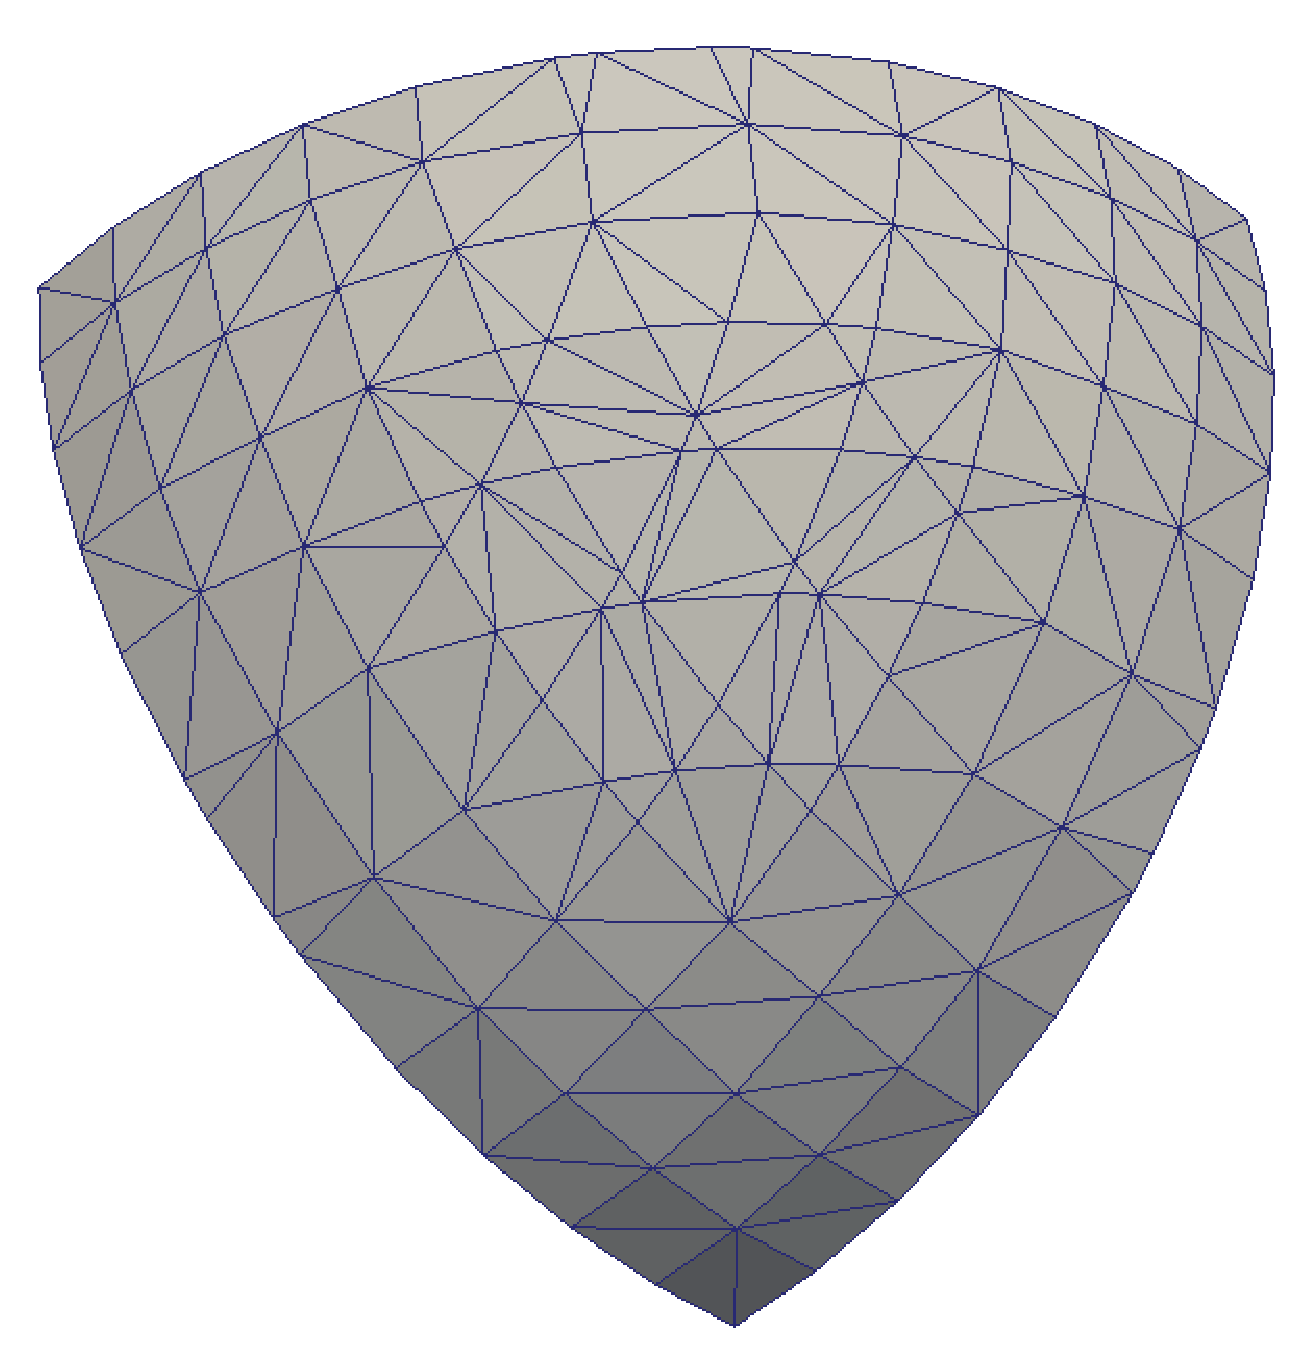
\includegraphics{octree/ex_images/hollow_sphere_1716_out.eps}
        }
    \end{subfigure}
    \begin{subfigure}[b]{0.49\linewidth}
        \scalebox{0.25}{
            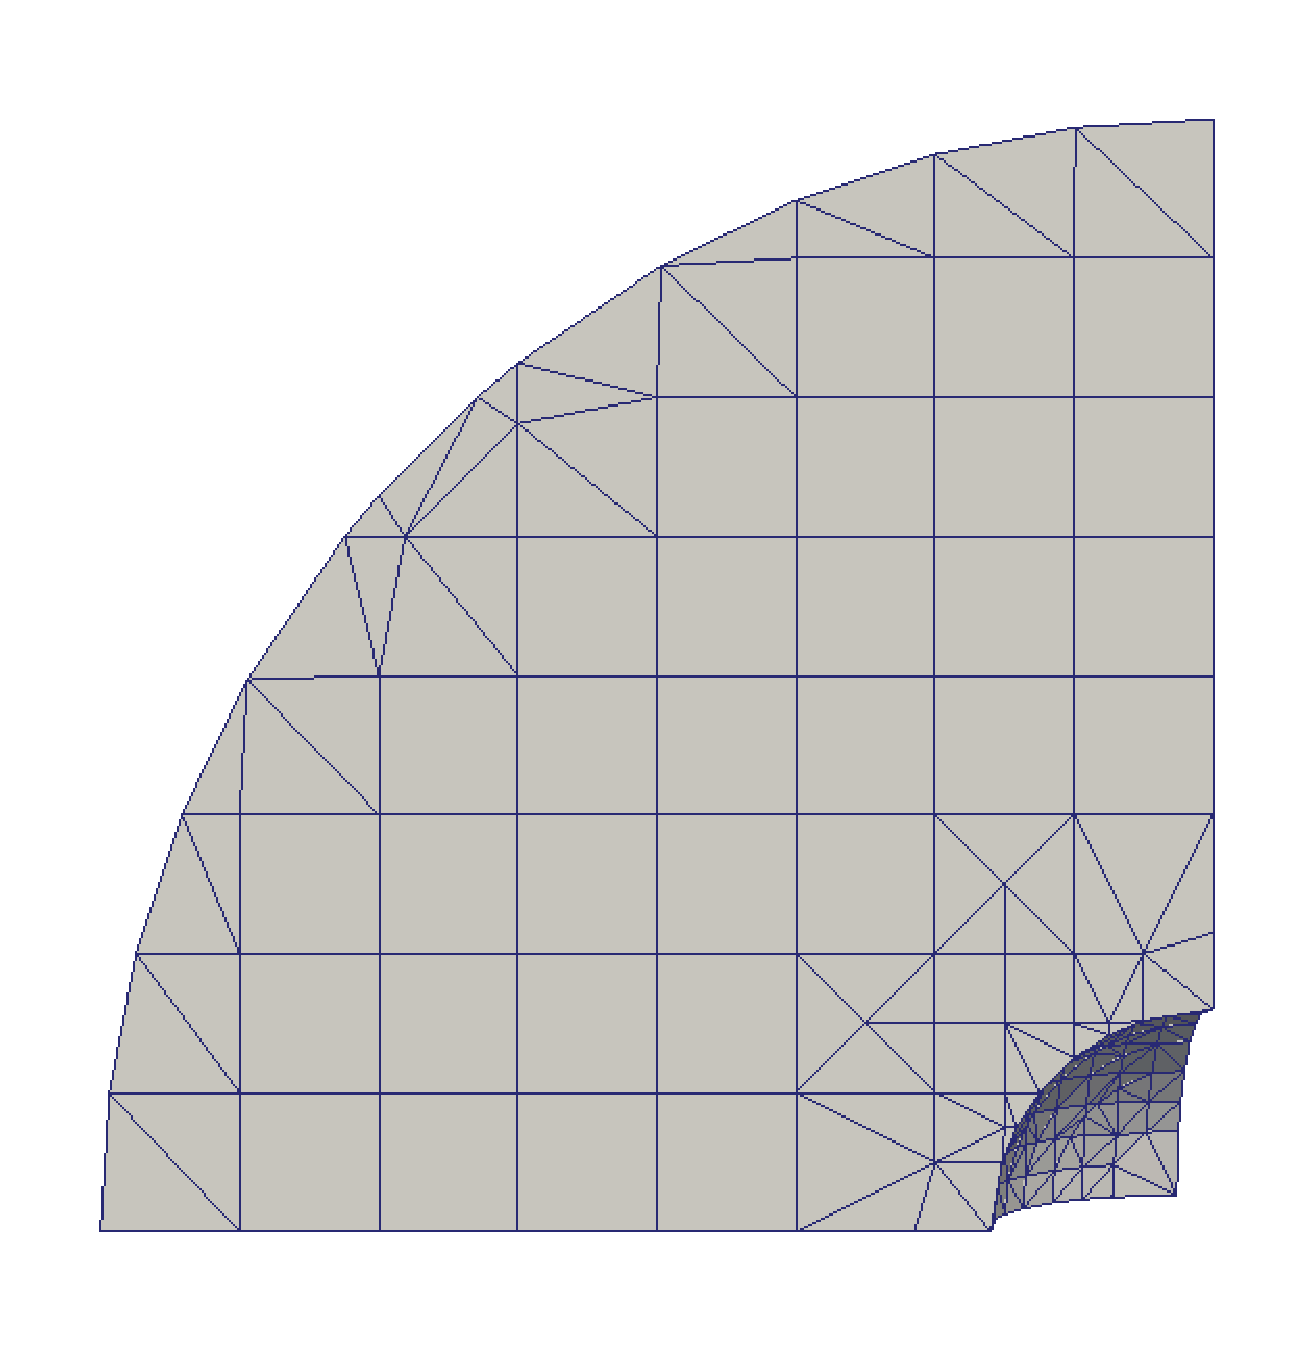
\includegraphics{octree/ex_images/hollow_sphere_1716_side.eps}
        }
    \end{subfigure}\\
    \begin{subfigure}[b]{1\linewidth}
        \centering
        \scalebox{0.5}{
            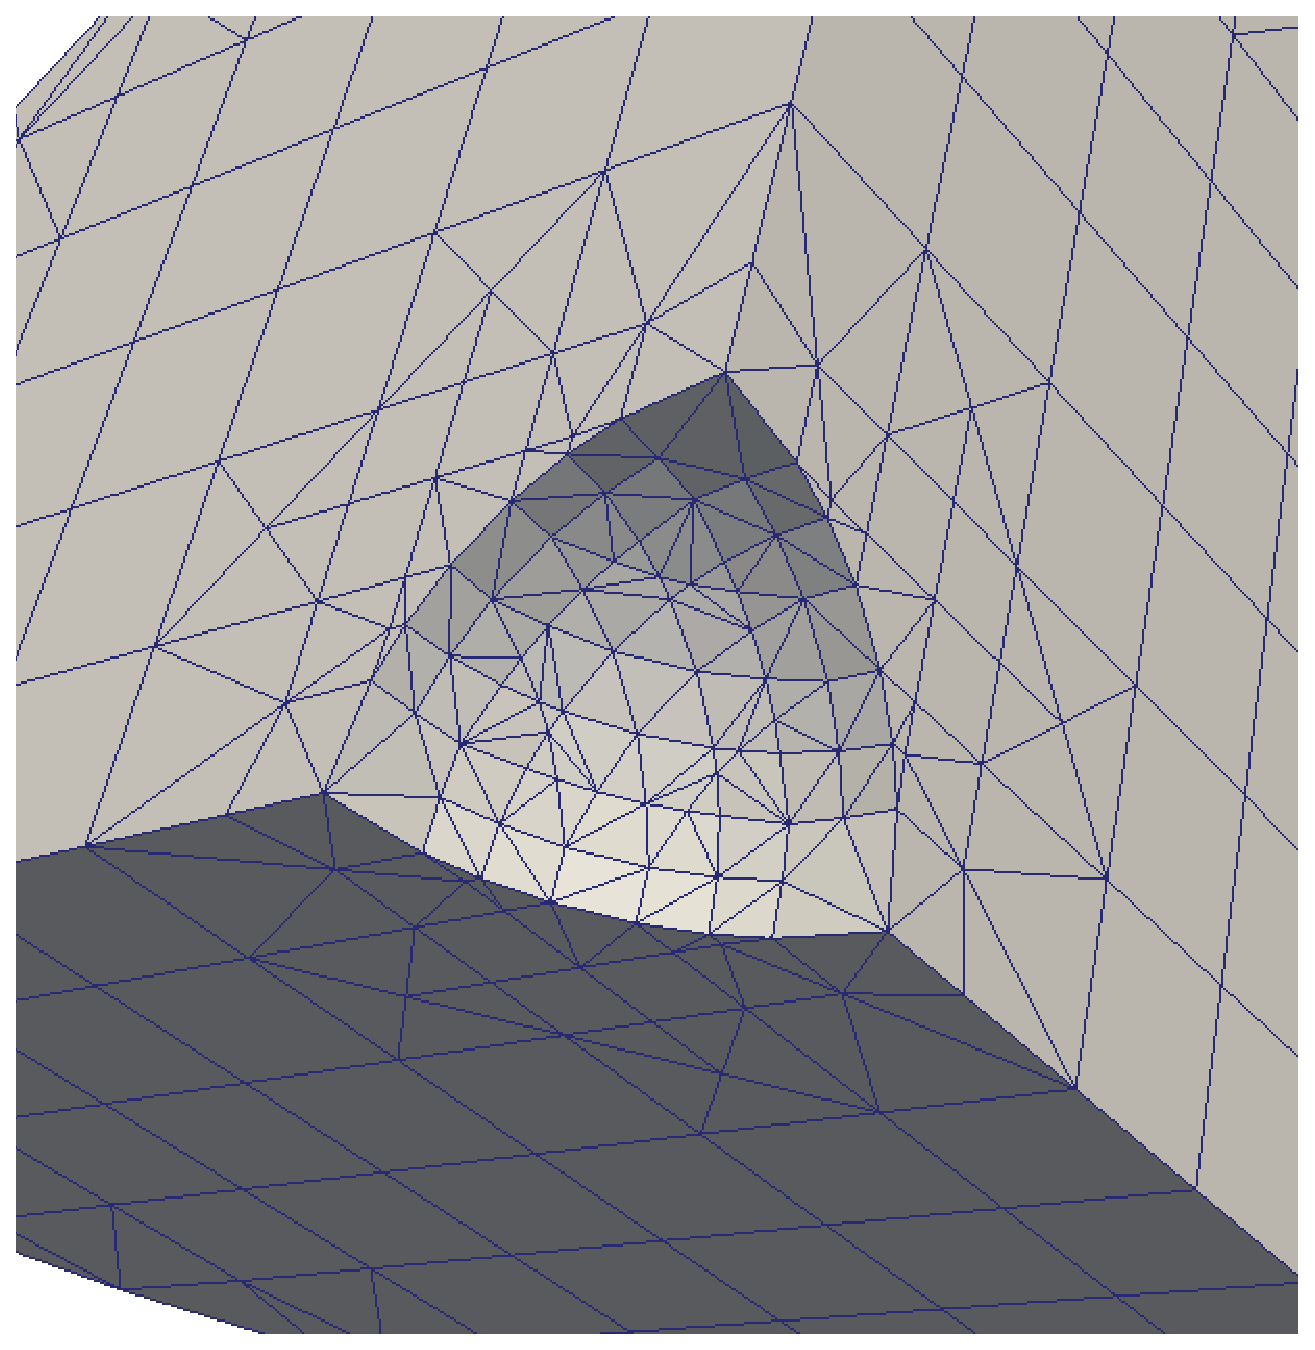
\includegraphics{octree/ex_images/hollow_sphere_1716_front.eps}
        }
    \end{subfigure}
    \caption{Mesh of the hollow sphere with 1716 DOFs}
    \label{oct_fig:ex_hollow_sphere_mesh_1716}
\end{figure}
\begin{figure}
    \centering
    \begin{subfigure}[b]{0.49\linewidth}
        \scalebox{0.25}{
            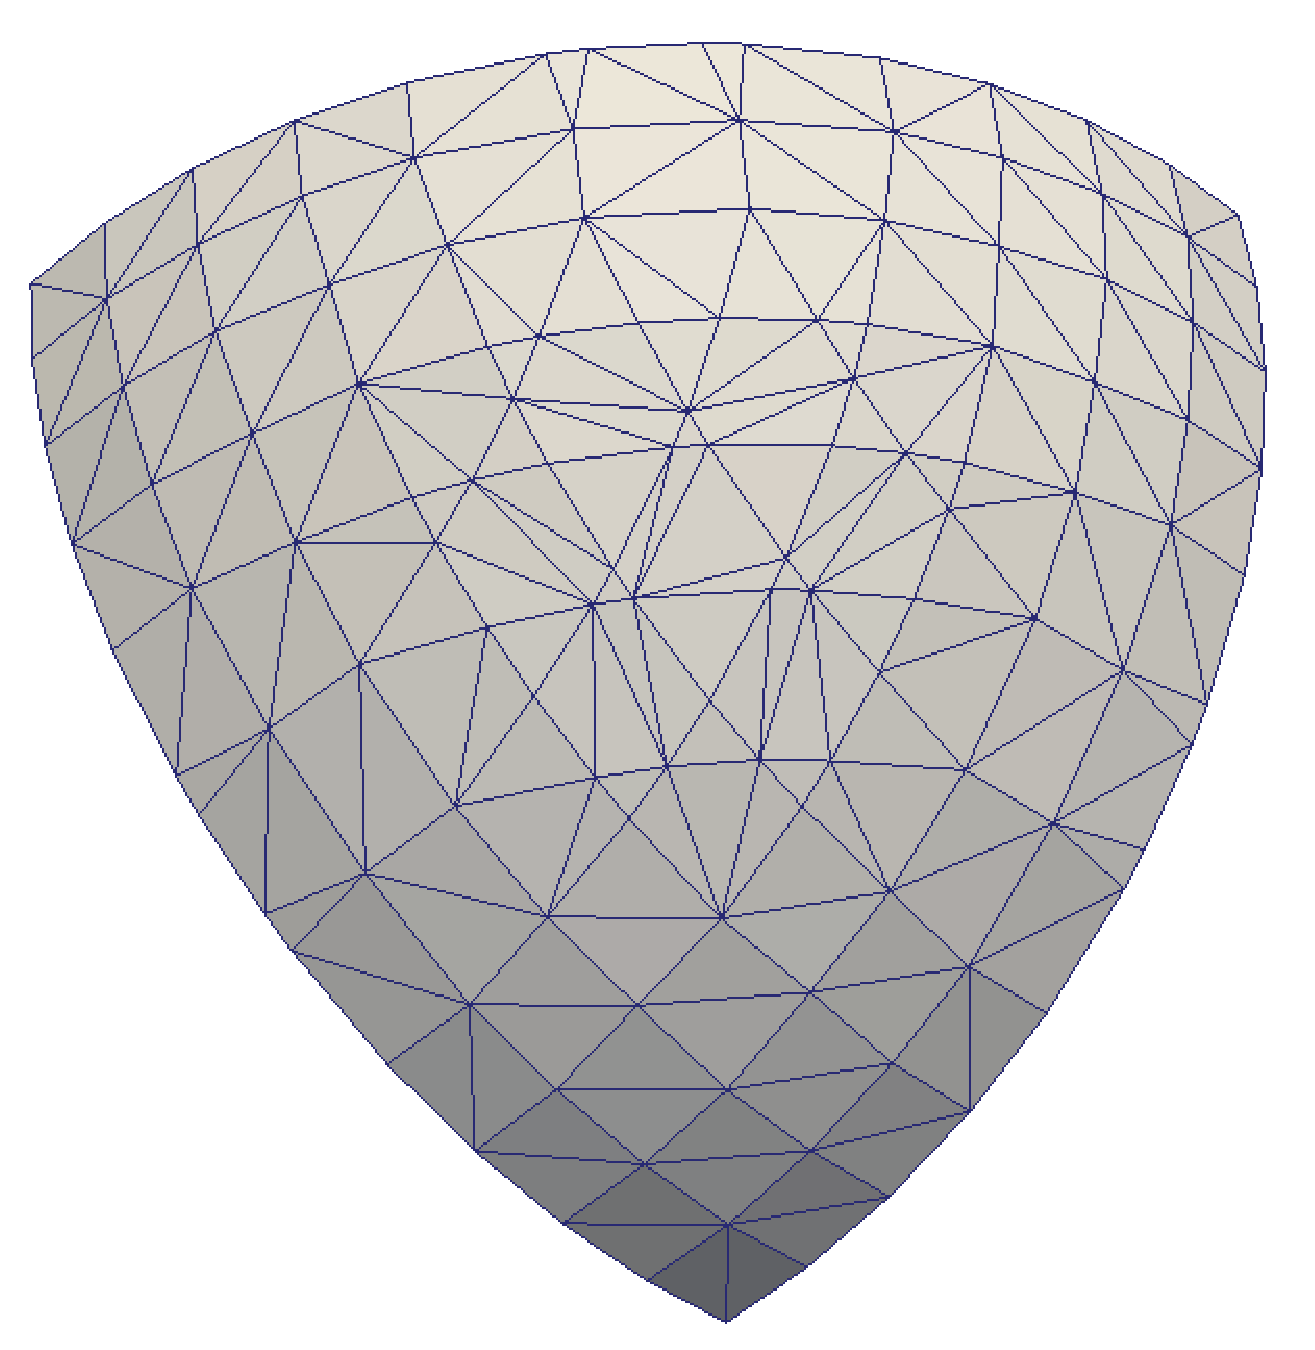
\includegraphics{octree/ex_images/hollow_sphere_3896_out.eps}
        }
    \end{subfigure}
    \begin{subfigure}[b]{0.49\linewidth}
        \scalebox{0.25}{
            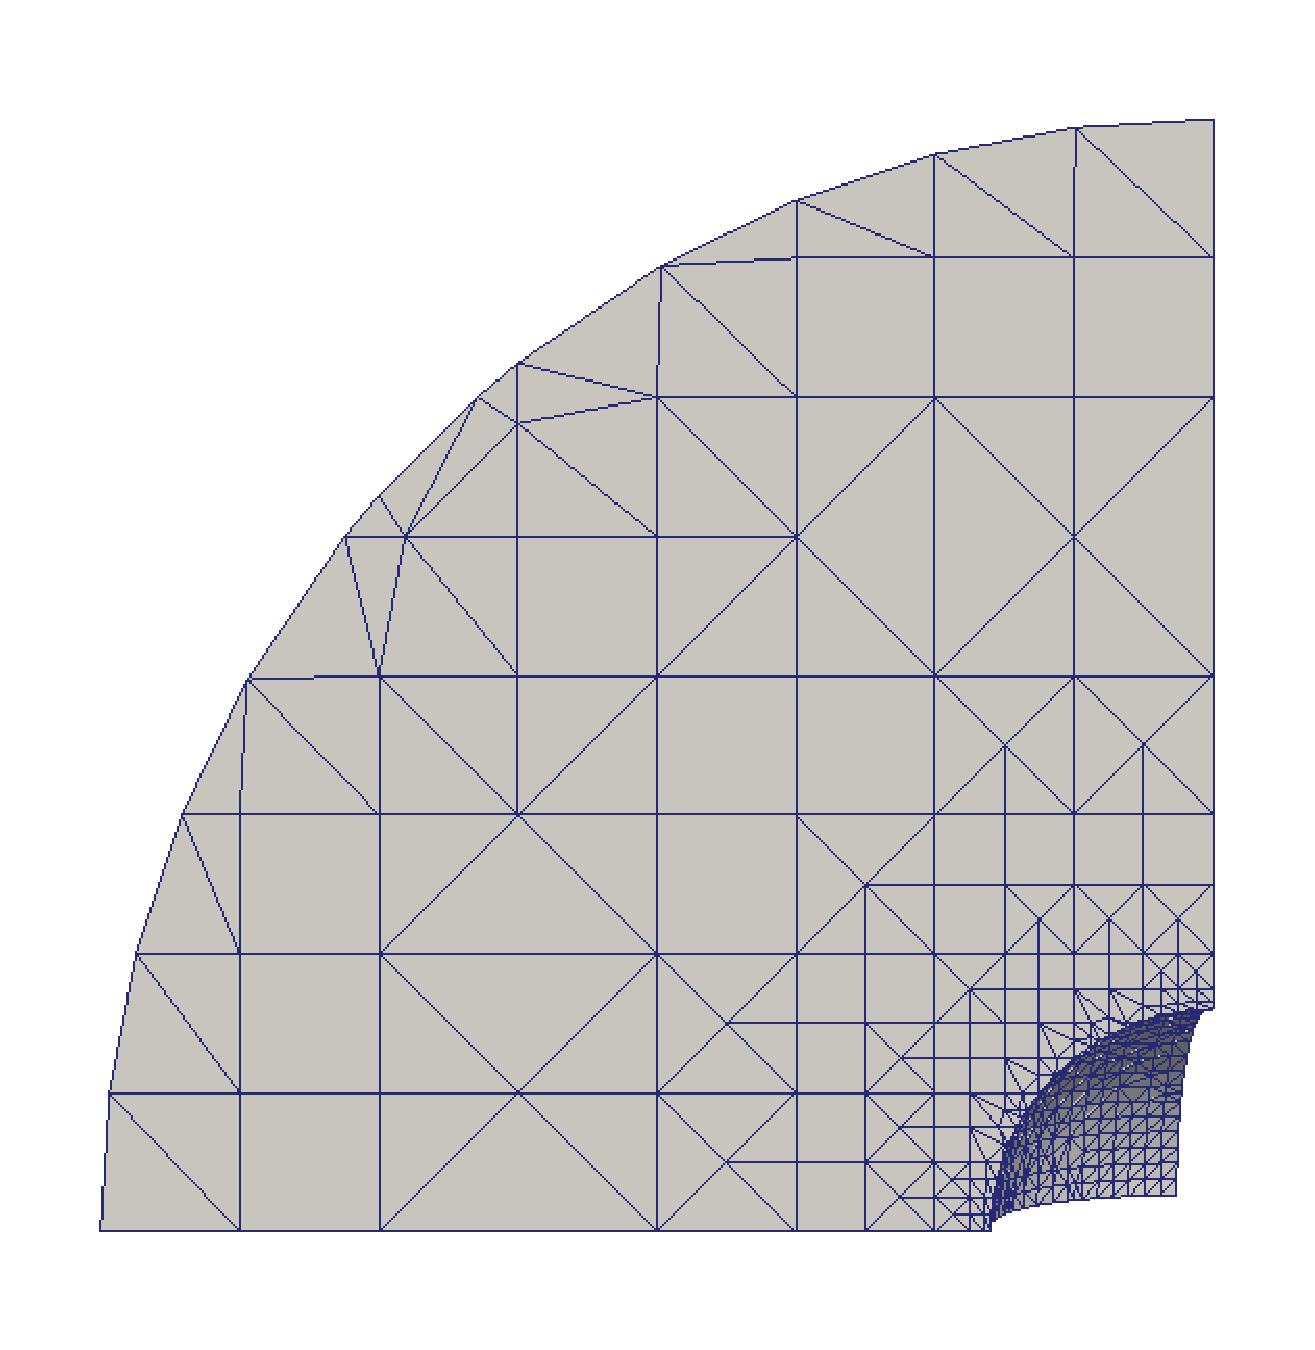
\includegraphics{octree/ex_images/hollow_sphere_3896_side.eps}
        }
    \end{subfigure}\\
    \begin{subfigure}[b]{1\linewidth}
        \centering
        \scalebox{0.5}{
            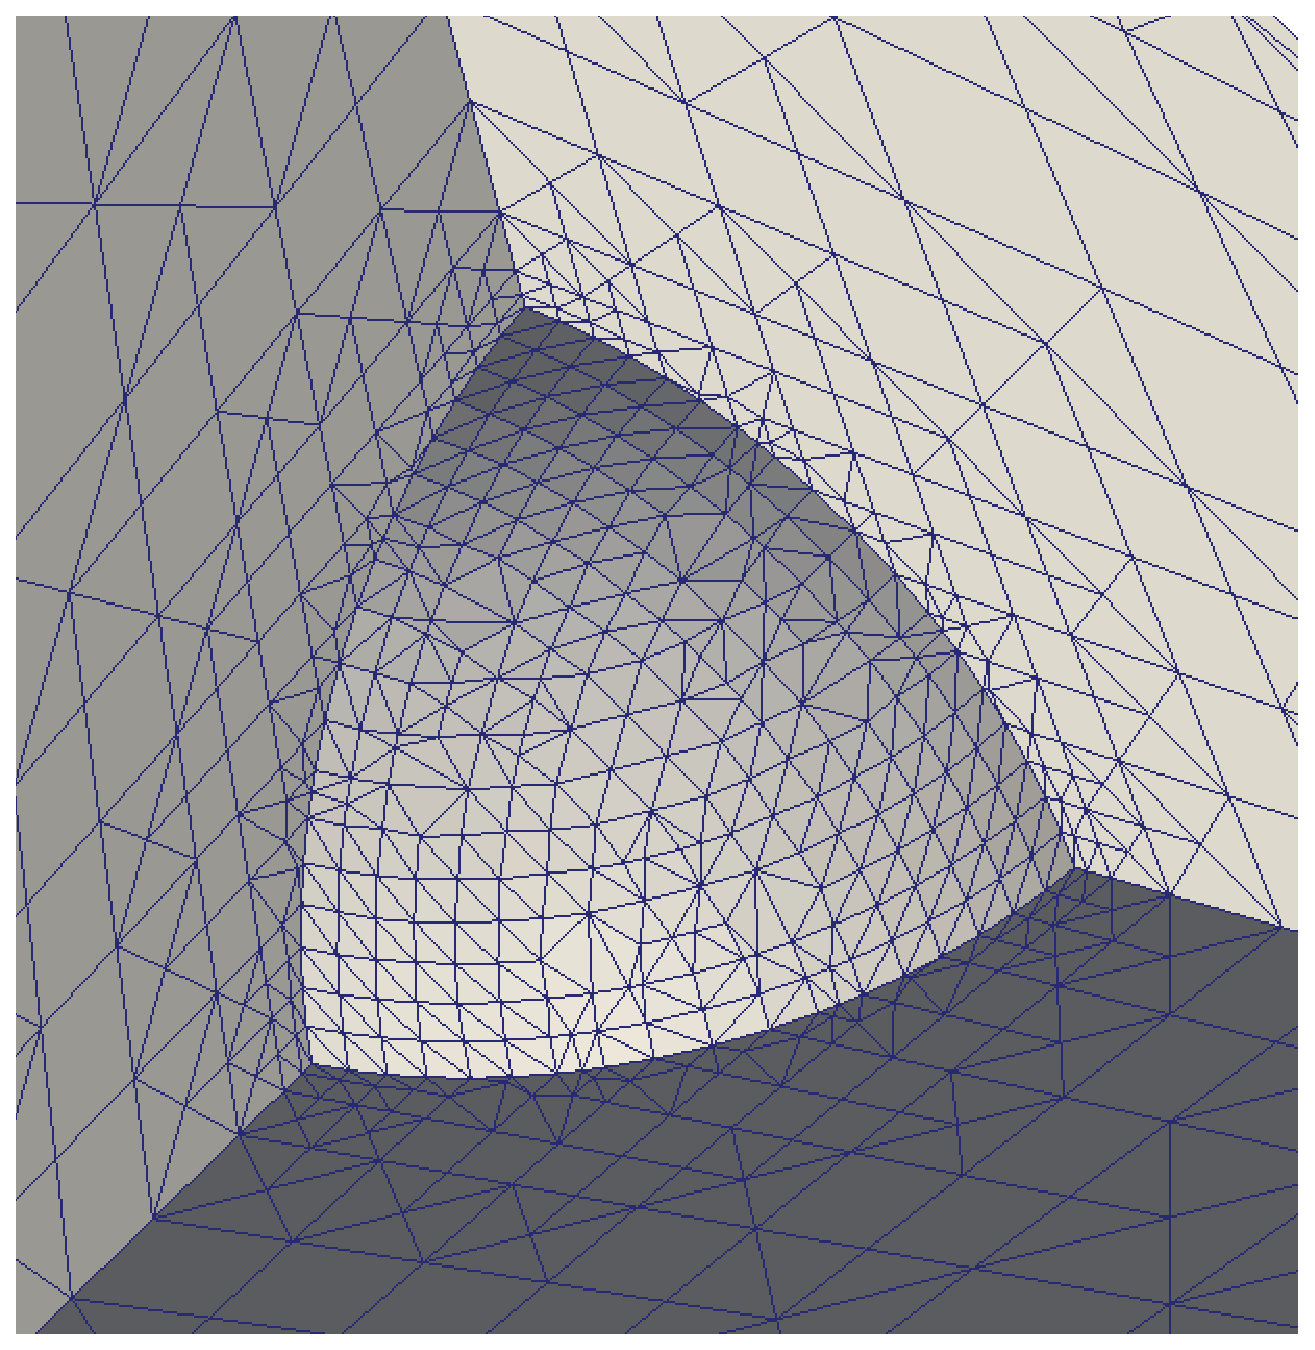
\includegraphics{octree/ex_images/hollow_sphere_3896_front.eps}
        }
    \end{subfigure}
    \caption{Mesh of the hollow sphere with 3896 DOFs}
    \label{oct_fig:ex_hollow_sphere_mesh_3896}
\end{figure}
\begin{figure}
    \centering
    \begin{subfigure}[b]{0.49\linewidth}
        \scalebox{0.25}{
            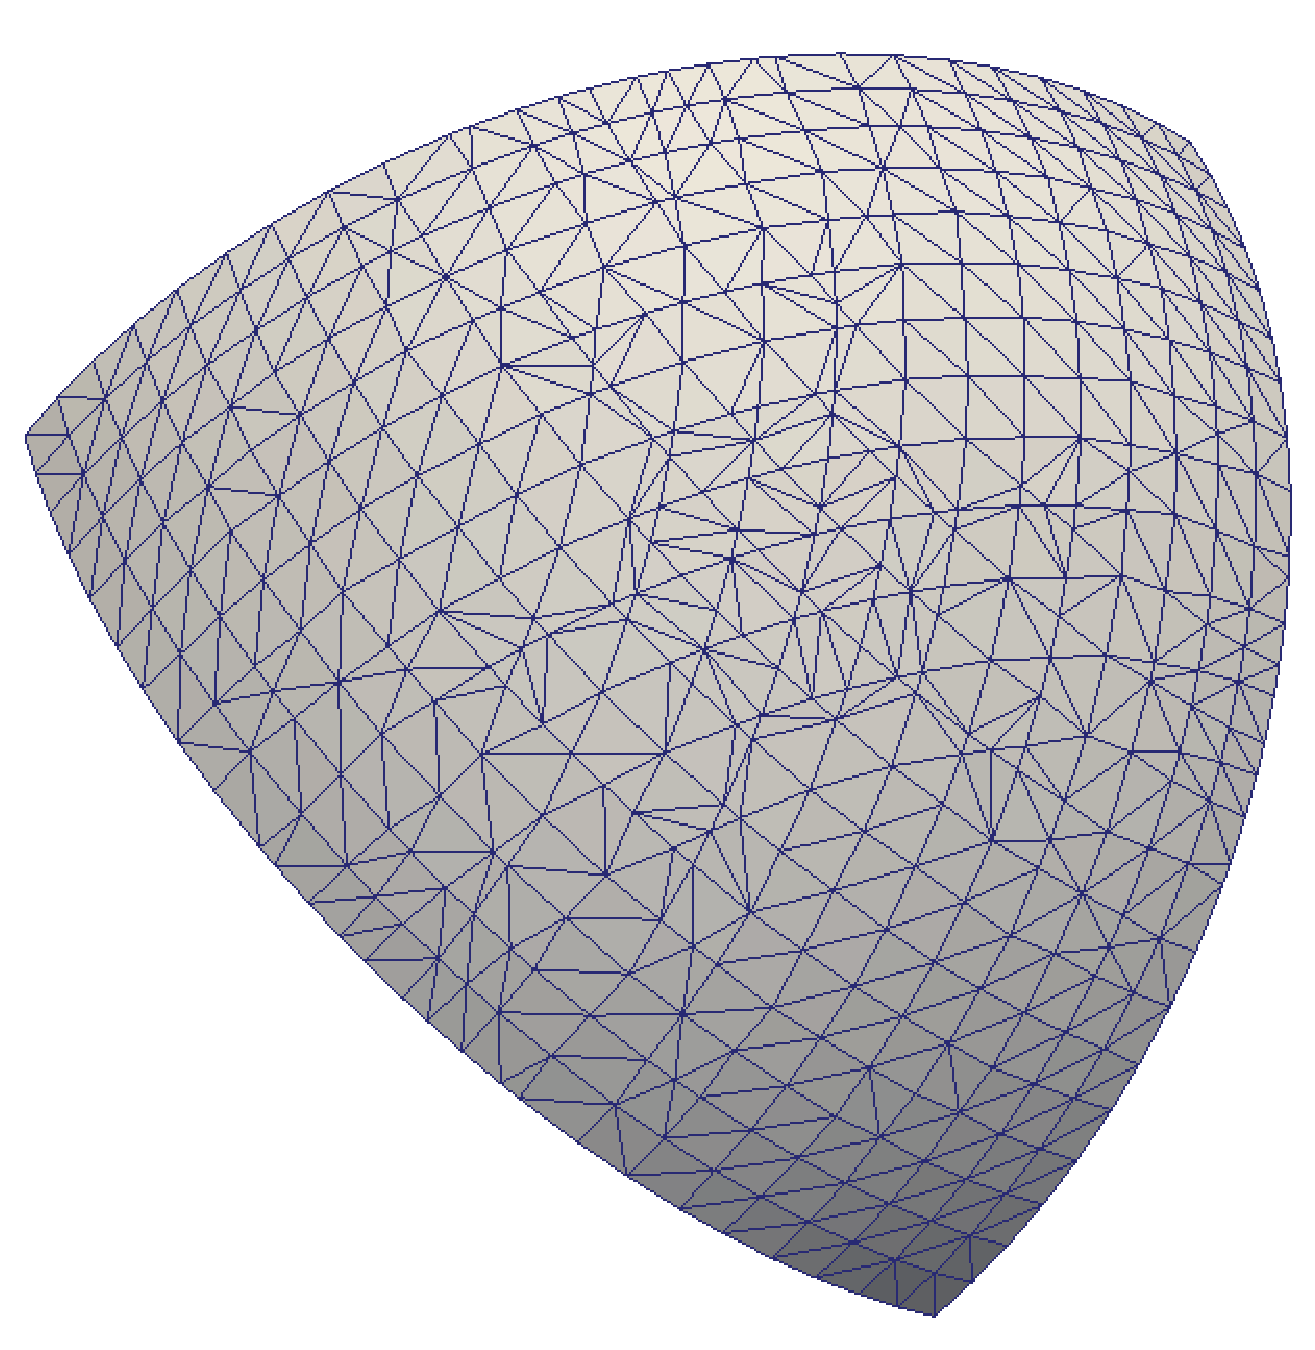
\includegraphics{octree/ex_images/hollow_sphere_12078_out.eps}
        }
    \end{subfigure}
    \begin{subfigure}[b]{0.49\linewidth}
        \scalebox{0.25}{
            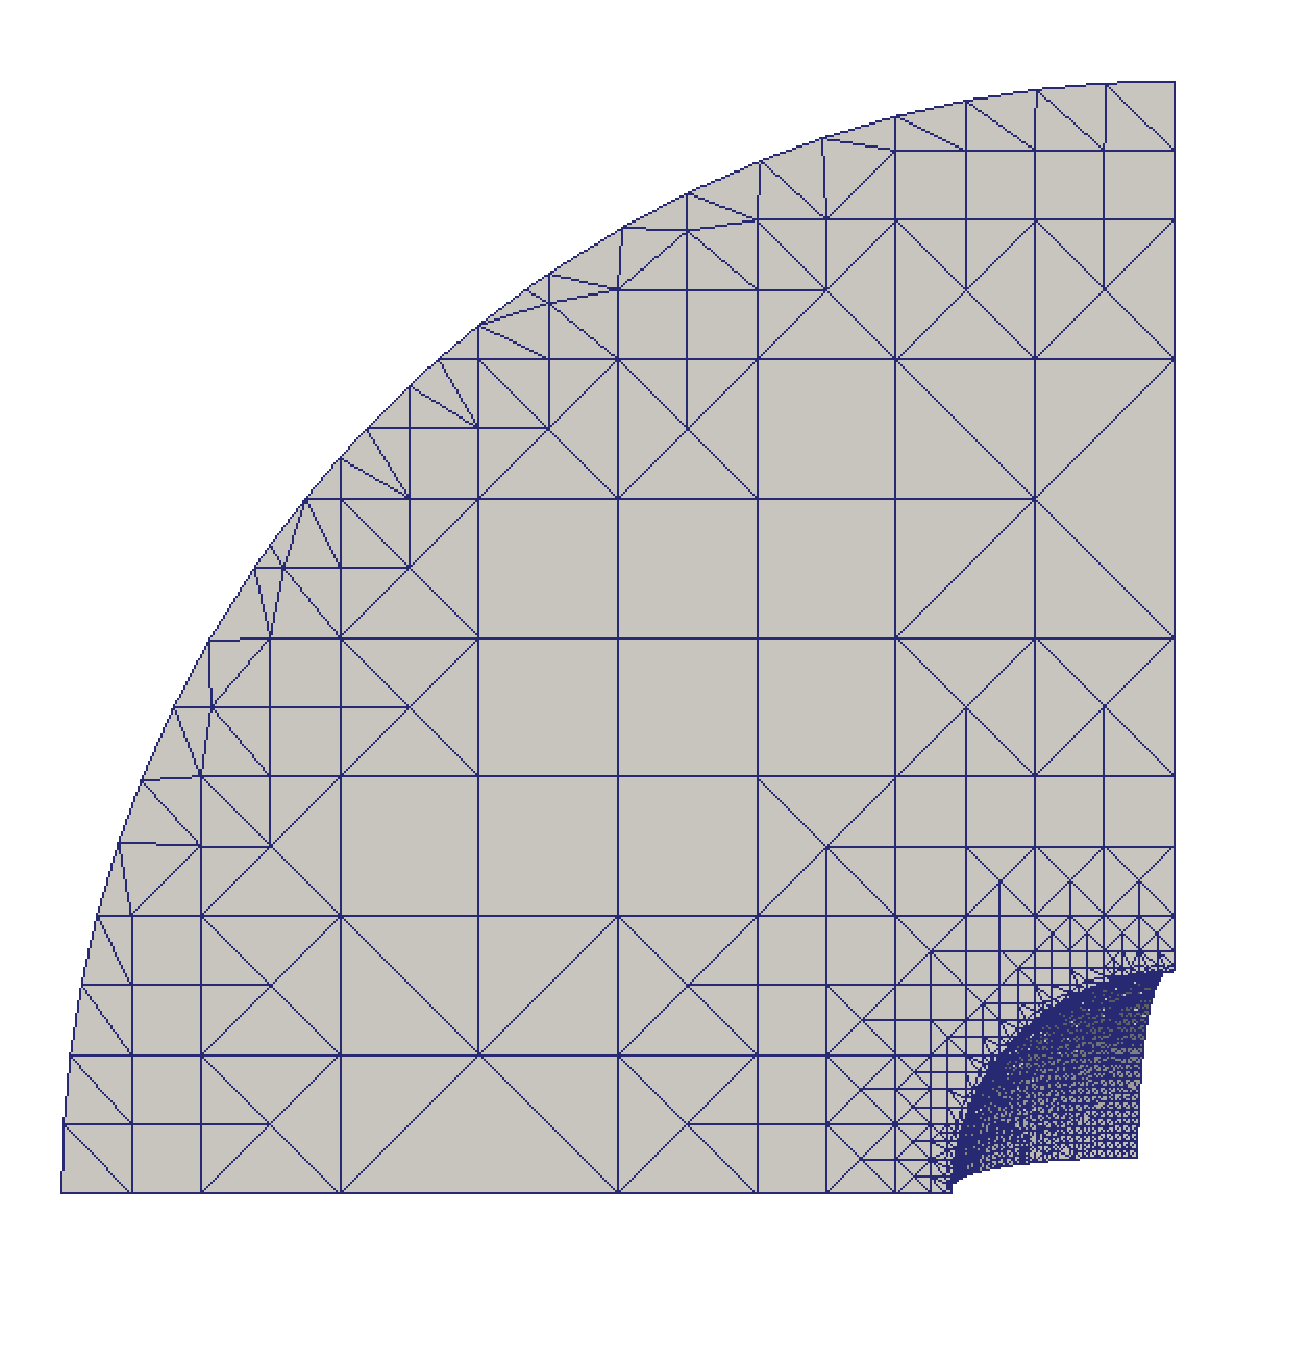
\includegraphics{octree/ex_images/hollow_sphere_12078_side.eps}
        }
    \end{subfigure}\\
    \begin{subfigure}[b]{1\linewidth}
        \centering
        \scalebox{0.5}{
            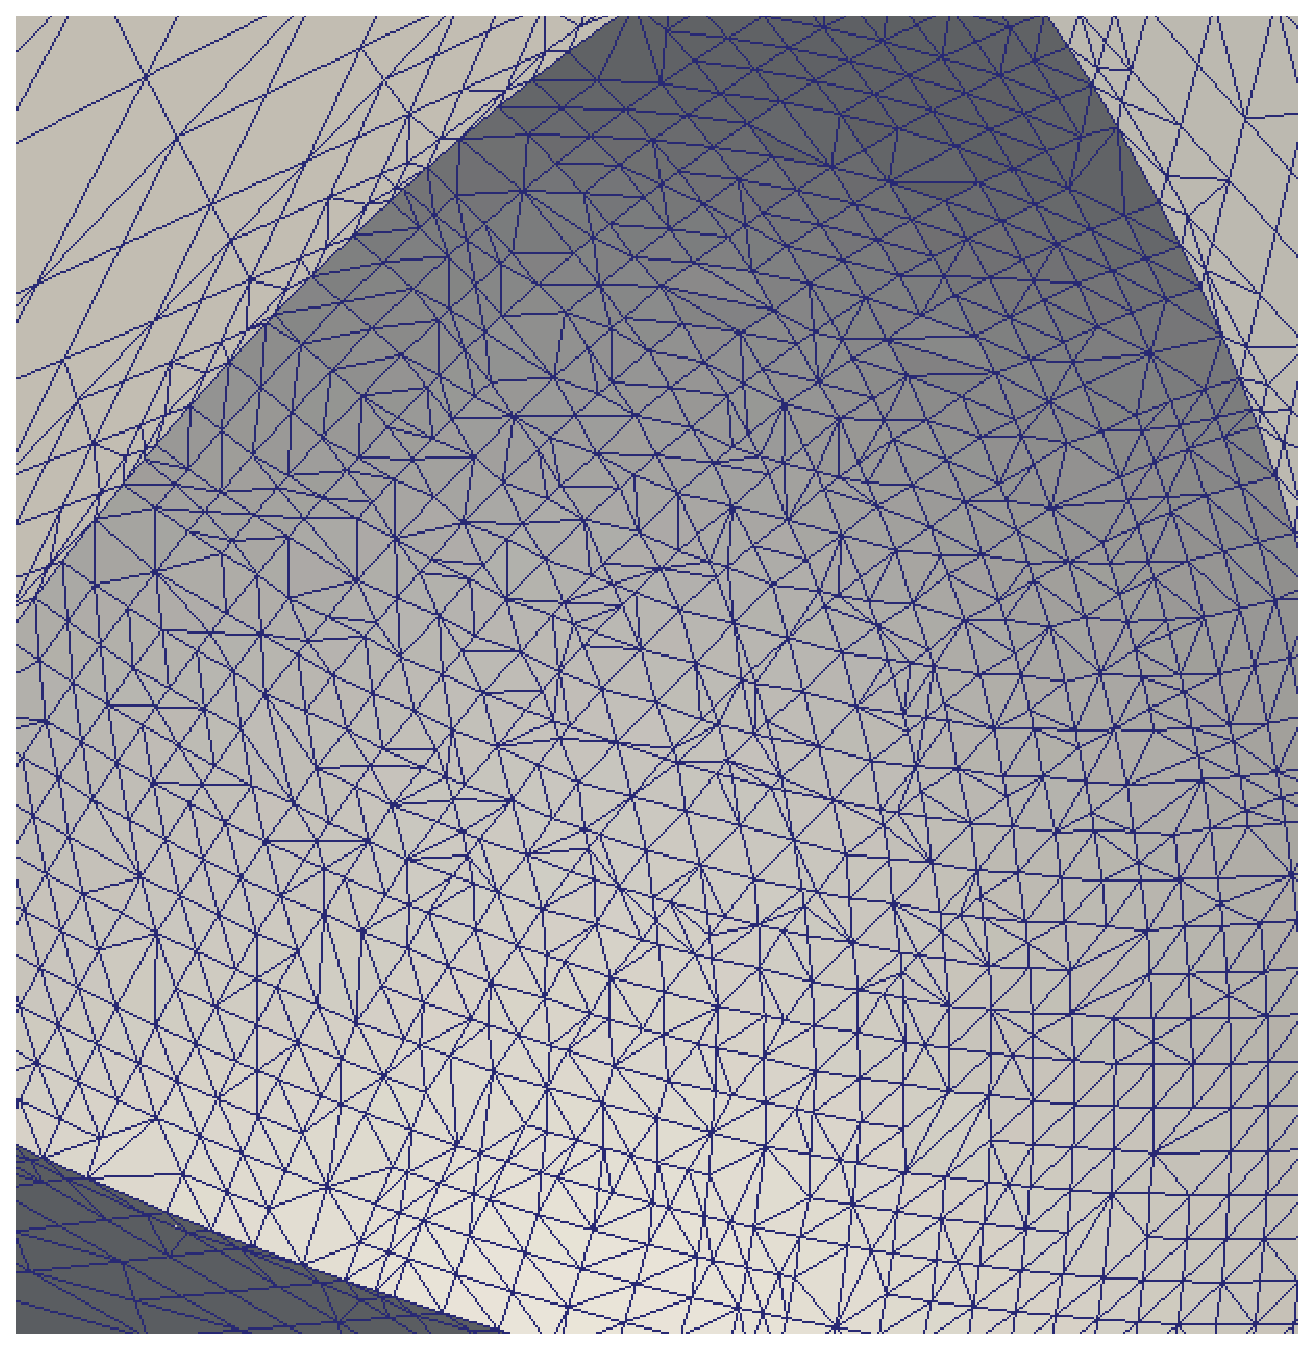
\includegraphics{octree/ex_images/hollow_sphere_12078_front.eps}
        }
    \end{subfigure}
    \caption{Mesh of the hollow sphere with 12078 DOFs}
    \label{oct_fig:ex_hollow_sphere_mesh_12078}
\end{figure}
% \begin{figure}[h!]
%   \centering
%   \scalebox{0.3}{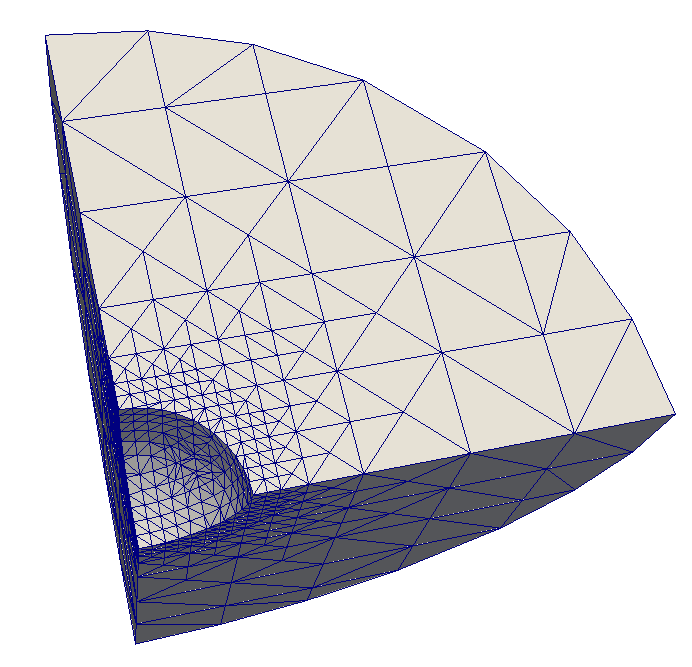
\includegraphics{octree/ex_images/oct_ex_mesh.png}}
%   \caption{Mesh of the hollow sphere}
%   \label{oct_fig:ex_hollow_sphere_meshP}
% \end{figure}

Stress boundary \hl{condition} in Eq.~\ref{oct_eq:ex_sphere_hole_bond_str} is applied on two spherical surfaces.
\begin{subequations}
    \begin{align}
    \sigma_{RR}(R=a,\phi,\theta) & = \frac{p_aa^3-p_bb^3}{b^3-a^3} - \frac{(p_a-p_b)b^3a^3}{(b^3-a^3)R^3}\\
    u_z(x,y,0) &= 0\\
    u_y(x,0,z) & = 0 \\
    u_x(0,y,z) & = 0
  \end{align}
\label{oct_eq:ex_sphere_hole_bond_str}
\end{subequations}
%
The convergence study is plotted in Fig.~\ref{oct_fig:ex_hollow_sphere_conv} and the mesh with corresponding DOFs are plotted in Fig.~\ref{oct_fig:ex_hollow_sphere_mesh_1716}, Fig.~\ref{oct_fig:ex_hollow_sphere_mesh_3896} and Fig.~\ref{oct_fig:ex_hollow_sphere_mesh_12078}
\begin{figure}[h!]
    \centering
    \scalebox{0.75}{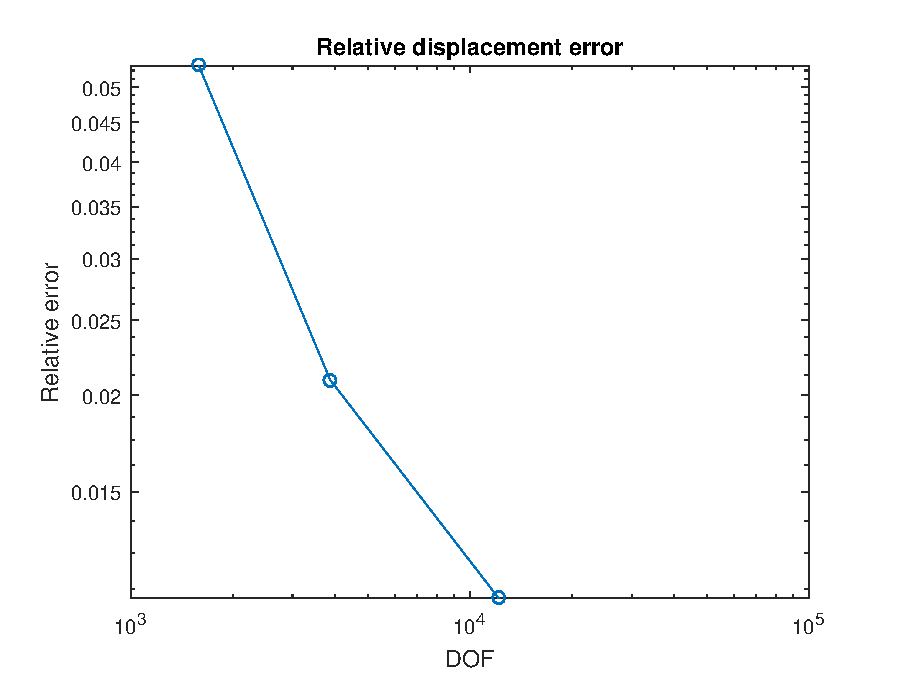
\includegraphics{octree/ex_images/ex_sphere_hole_conv.eps}}
    \caption{Convergence of displacement error}
    \label{oct_fig:ex_hollow_sphere_conv}
\end{figure}